\documentclass{article}

\usepackage[a4paper]{geometry}
\usepackage{graphicx}
\usepackage[utf8]{inputenc}
\usepackage{subcaption}
\usepackage{placeins}
\usepackage{wrapfig}
\usepackage{float}
\usepackage{hyperref}


\graphicspath{{./images/}}

\title{\textbf{WizardGame 2}}
\author{
    Dumitru Mițca\\
    Grupa NNNNL}
    \date{2023}

    \begin{document}
    \maketitle

    \hypersetup{linkbordercolor=1 1 1}
    \renewcommand*\contentsname{Cuprins}
    \tableofcontents
    \hypersetup{linkbordercolor=1 0 0}


    \newpage

    \section{Contextul jocului}
    WizardGame 2 este un sequel la \href{https://github.com/RealKC/WizardGame}{WizardGame}
    \footnote{Acesta a fost proiectul meu pentru POO, un sumar al poveștii veți
    regasi in \href{sec:anexa1}{Anexa 1}}.
    Dupa evenimentele \emph{WizardGame} în care Mircea l-a înfrânt pe Adrian, Mircea decide sa se
    mute la casa lui de pe Bulevardul Magheru din București, deoarece Brăila îi aduce amintiri
    triste.

    Cristian, fratele lui Adrian și necromant\footnote{Un vrăjitor care deține puteri ce
    îi permit să reînvie și să controleze morții.} renumit, care era plecat în Sicilia
    pentru a învăța vrăji de la magicienii sicilieni este anunțat de moarte fratele său
    și jură că îl va răzbuna. În următorii 2 ani, Cristian stabilizează clanul Isch'tauk,
    care devenise haotic după moartea lui Adrian, fostul lider, și se pregătește pentru
    răzbunare. Iar pe data 25 octombrie 1966 își pune în acțiune planurile.

    În dimineața acestei zile Cristian își aduce armate de nemorți, în care sunt și Matei
    și Adrian, reînviați de Cristian, și pe cei mai buni dintre discipolii lui \emph{Denis,
    the Cosmicbane} și \emph{Cezar, the Tătărașiborn Guardian} în București și astfel
    începe atacul asupra lui Mircea.

    În timpul luptei, \emph{Eduard, the Carpathian Thunder} aude lupta ce se întâmplă în jurul
    casei sale, și decide și el să lupte împotriva armatei nemoarte.

    \section{Gameplay și interacțiunea jucătorului cu jocul}

    \begin{figure}[h]
        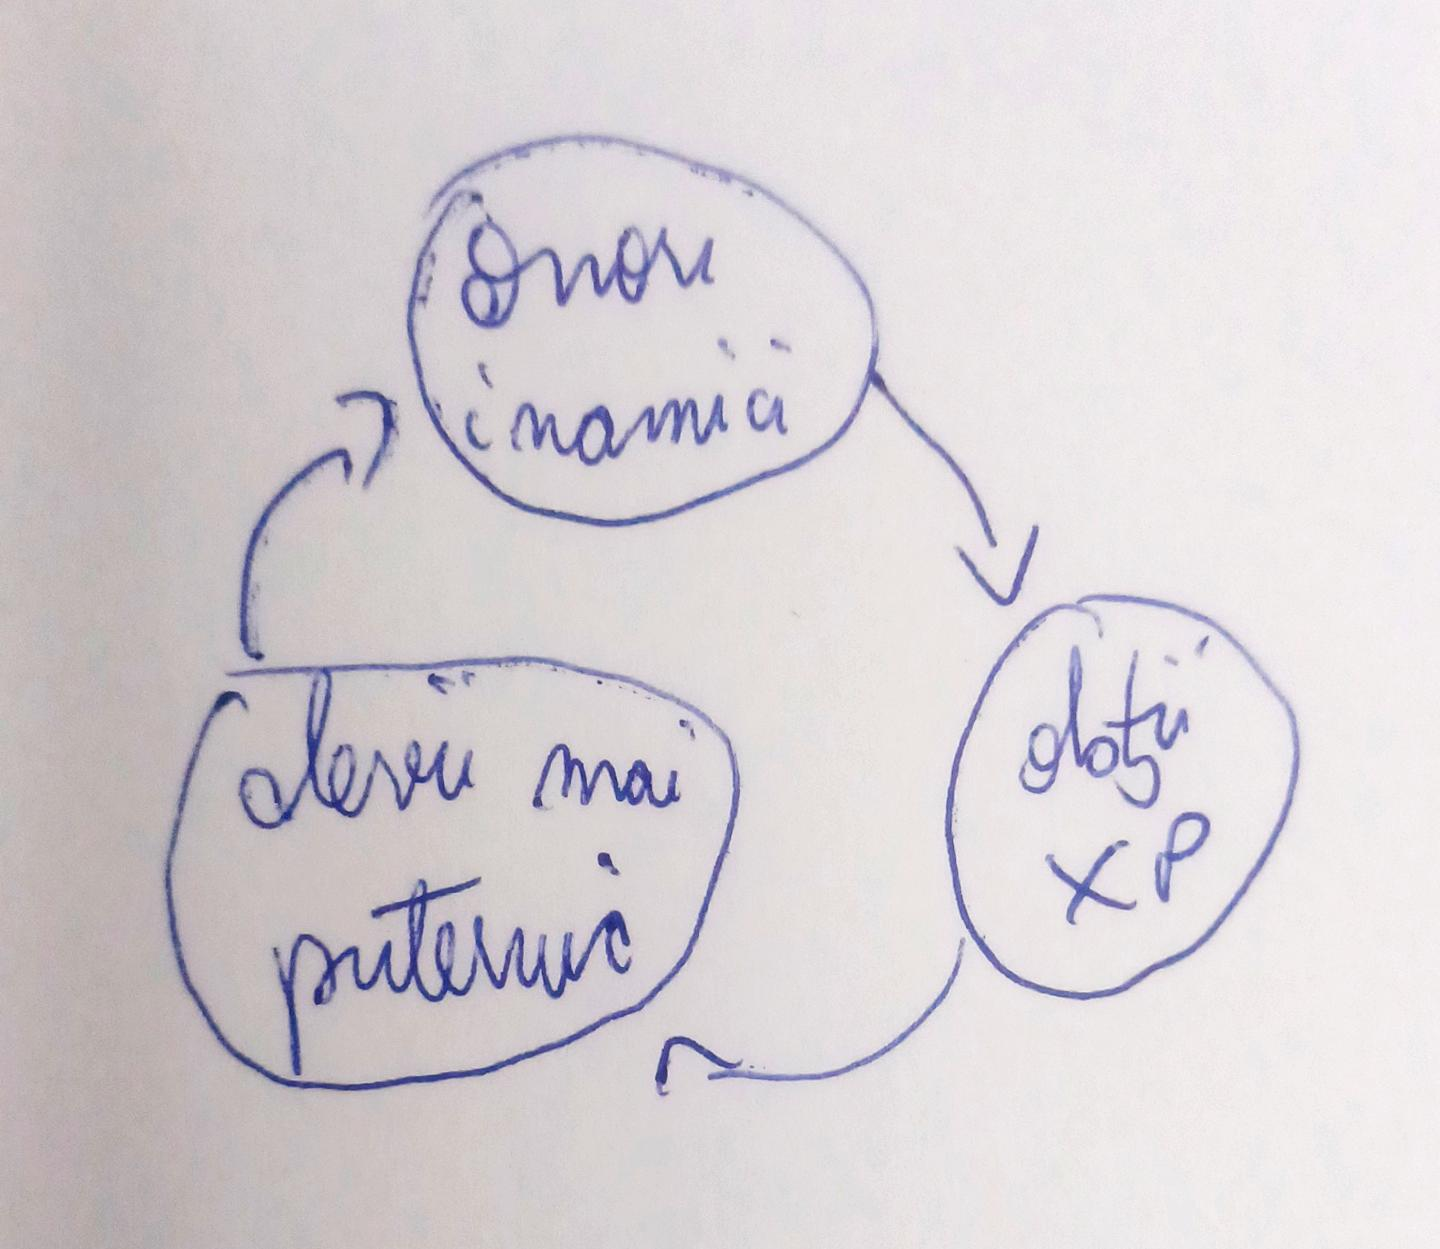
\includegraphics[scale=0.125]{gameplayloop}
        \centering
        \caption{WizardGame 2 Gameplay loop}
    \end{figure}

    După ce jucătorul își alege un personaj \ref{sec:pcs} și intră într-un nivel, dispune
    doar de un singur atac: o vrajă specifică acelui personaj. Cât timp jucătorul se află
    în nivel, acesta va doborî inamici, care vor lăsa la poziția lor \emph{experiență}.
    Colectarea \emph{experienței} va duce eventual la creșterea nivelului jucătorului, lucru
    care îi va permite să obțină arme sau vrăji noi, sau să își îmbunătățească caracteristicile
    \ref{sec:stats}.

    Extensii asupra sistemului acesta sunt discutate după prezentarea armelor, vrăjilor și
    echipamentului \ref{sec:exts}.

    Completarea unui nivel necesită învingerea boss-ului acelui nivel. Boss-ul apare la
    minutul 20:00\footnote{Dacă pe parcursul procesului de dezvoltare observ că 20 de
    minute este prea mult pentru un nivel, timpul va fi scurtat, dar nu la mai puțin de
    14 minute.} și trebuie învins pentru a progresa la nivelul următor.

    Jucătorul își mișcă personajul folosing tastele W (în sus), S (în jos), A (la stânga) și D
    (la dreapta), iar abilitățile sale sunt activate automat, după un timer. Abilitățile care
    țintesc într-o direcție anume vor folosi direcția în care se mișcă jucătorul în momentul
    activării abilității. Atfel dificultatea jocului nu reiese din abilitatea jucătorului de a lovi
    inamicii, ci din abilitatea sa de a se feri de ei, sau atacurile lor, ceea ce va deveni dificil
    cu cât jucătorul se află mai mult într-un nivel.

    Sistemul de save/load al jocului este automat, și nu necesită o interacțiune explicită a
    jucătorului, dar o idee interesantă ar fi introducerea conceptului de "save slot". Acesta ar
    permite jucătorului să asocieze un save cu un "slot", permițându-i astfel să reia jocul de la
    început fără să ia acțiuni externe jocului. Prezența sistemului "save slot" ar introduce un motiv
    bun de a integra statistici despre un save în joc, dar nu m-am hotorât asupra prezenței acestui
    sistem și acest lucru v-a fi hotorât de constrângerile de timp.

    \section{Conținut}

    \emph{WizardGame 2} conține o varietate de inamici ce trebuie învinși de
    jucător și o varietate de vrăji și atacuri ce pot fi folosite de acesta pentru a ajunge
    la victorie.

    \label{sec:sprites}
    \begin{figure}[h]
        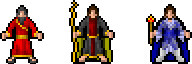
\includegraphics[scale=2]{player-characters}
        \centering
        \caption{Protagoniștii, de la stânga la dreapta: Mircea, Eduard, Mihai}
    \end{figure}

    Jucătorul poate alege între trei personaje: \emph{Mircea, The Wizard of Brăila},
    \emph{Mihai, the Fullmetal Wizard} și \emph{Eduard, the Carpathian Thunder}.
    \begin{itemize}
        \item \emph{Mircea} --- începe cu o vrajă care îi permite să arunce bile de foc
        \item \emph{Mihai} --- deoarece și-a pierdut brațul în Războiul Magilor din 1959,
        și-a implatat un braț magic metalic. Acesta îl face să fie mai slab cu atacuri
        magice, dar mai priceput cu atacuri ce presupun aruncarea unui obiect.
        \item \emph{Eduard} --- un vrăjitor cu control asupra fulgerului, astfel atacul
        său este un fulger. Jucătorul deblochează accesul la acest personaj după ce
        învinge primul nivel. Datorită reflexelor sale excelente, el are șansa atacului critic crescută.
    \end{itemize}

    Jucătorul poate folosi maxim 3 din urmatoarele vrăji și arme:
    \begin{itemize}
        \item \emph{Defendere Magi} --- o carte de vrăji care creează o zonă circulară în jurul
        jucătorului care rănește inamicii.
        \item \emph{Circulus Glaciei} --- o carte de vrăji care creează un cerc de țurțuri în jurul
        jucătorului.
        \item \emph{Ignis Respiratio} --- o carte de vrăji care creează o flacară în direcția în
        care se mișcă jucătorul.
        \item \emph{Terra Gutta} --- o carte de vrăji care creează blocuri de pământ în locații
        aleatoare pe hartă.
        \item \emph{Vortex Mercurius} --- o carte de vrăji care creează tornade ce pleacă de la
        jucător într-o direcție aleasă aleator.
        \item \emph{Pistol Carpați} --- un pistol, viteza sa de atac este crescută comparativ cu
        folosirea unei vrăji.
        \item \emph{Baltagul Vitoriei} --- un topor gigant, care pleacă în spirală de la jucător.
        spre exterior.
        \item \emph{Morning Star} --- o bila metalică cu țepi atașată cu un lanț de un mâner, se
        rotește în jurul jucătorului.
        \item \emph{Holy Lamp} --- crează o arie conică în fața jucătorului care are bonus de putere
        împotriva inamicilor nemorți.
    \end{itemize}

    Jucătorul poate echipa maxim 3 din următoarele seturi de echipament, care îi vor conferi
    efecte pasive:
    \begin{itemize}
        \item \emph{Fluierul Sfintei Vineri} --- oferă un bonus vitezei jucătorului.
        \item \emph{Colier cu Safir} --- oferă un bonus puterii magicii jucătorului.
        \item \emph{Glasses of Infirma Aspectu} --- crește șansa atacului critic.
        \item \emph{Cape of Great Magic} --- crește puterea magică a jucatorului, dar scade viteza
        de atac.
        \item \emph{Orichalcum Magnet} --- crește raza de pickup a jucătorului.
        \item \emph{Mănușile Alchimistului Focului} --- oferă un bonus puterii magicii jucătorului,
        crescut față de \emph{Colierul cu Safir}, dar va scădea raza de pickup. Bonusul v-a fi mai
        mare când sunt folosite de \emph{Mircea}.
        \item \emph{Chainmail Shirt} --- permite jucătorului să supraviețuiască mai multor atacuri
        înainte de a muri.
        \item \emph{Ring of Anima} --- permite jucătorului să-și regeneze viața pierdută.
        \item \emph{Cercei cu Rubine} --- crește viteza de atac a jucătorului.
    \end{itemize}

    Personajul jucătorului are următoarele caracteristici, care pot fi îmbunătățite pe parcursul
    jocului:
    \begin{itemize} \label{sec:stats}
        \item viața (\textbf{HP}) --- se referă la câte atacuri poate jucătorul suferi înainte de a muri.
        \item puterea magică (\textbf{+ATK\%}) --- un bonus procentual aplicat asupra unui atac normal.
        \item șansa atacului critic (\textbf{CRIT\%}) --- șansa ca un atac să își aibă valoare dublată.
        \item viteza (\textbf{+SPD\%}) --- cât de rapid se mișca personajul jucătorului.
        \item raza de pickup (\textbf{+PCK}) --- raza maximă în care trebuie să se afle un item
        pe hartă pentru a putea fi luat de jucător, măsurată în pixeli.
        \item viteza de atac (\textbf{+HST\%}) --- cât de rapid atacă jucătorul.
    \end{itemize}
    \label{sec:pcs}

    Cele enumerate mai sus ar fi obținute de jucător în momentul în care și-a crescut nivelul,
    fiindu-i puse la dispoziție o alegere între arme, vrăji, echipament și posibilitatea de a
    crește valoarea unei caracteristici.

    \label{sec:exts}
    Câteva idei care ar adaugă mai multă adâncime acestor sisteme ar fi posibilitatea îmbunătățirii
    vrăjilor, armelor și echipamentului prin creșterea nivelelor acestora folosind un sistem de
    nivele pe iteme și existența unui sistem de îmbunătățiri permanente, înafara nivelelor.
    Prezența acestor sisteme în jocul final nu este decisă încă și va fi hotărâtă de timpul
    disponibil în momentul implementării jocului.

    Jucătorul va trebuie să lupte cu inamici simpli (zombie, scheleți, fantome), cu inamici de tip
    mini-boss, care sunt doar versiuni mai mari și mai puternici a celor simpli, și cu inamici de
    tip boss, care sunt următorii și care sunt importanți poveștii jocului:
    \begin{itemize}
        \item \emph{Matei, the Prophaned} --- sensei-ul lui Mircea, a murit în \emph{WizardGame}, dar a
        fost reînviat de Cristian pentru a ajuta în răzbunarea lui. Puțin rămâne din shamanul care
        a fost Matei în viață. Matei folosește magia umbrelor, învățată de el în timpul Războiului Magilor.
        \item \emph{Adrian, the Crimson Undead} --- fostul lider al clanului Isch'tauk și fratele
        lui Cristian. Se pare că doliul l-a dus pe Cristian să facă acte de neiertat propriei familii.
        \item \emph{Cezar, the Tătărașiborn Guardian} --- unul dintre cei mai buni discipoli ai lui
        Cristian, născut în Tătărași.
        \item \emph{Denis, the Cosmicbane|} --- unul dintre cei mai buni discipoli ai lui Cristian, și
        mag cu puteri spațiale, specialitățile lui sunt teleportarea și invizibilitatea.
        \item \emph{Cristian, the Necromancer of Neamț} --- caută să își răzbune fratele. Jucătorul va
        lupta cu el în două faze.
    \end{itemize}


    \section{Niveluri}

    \begin{figure}[h]
        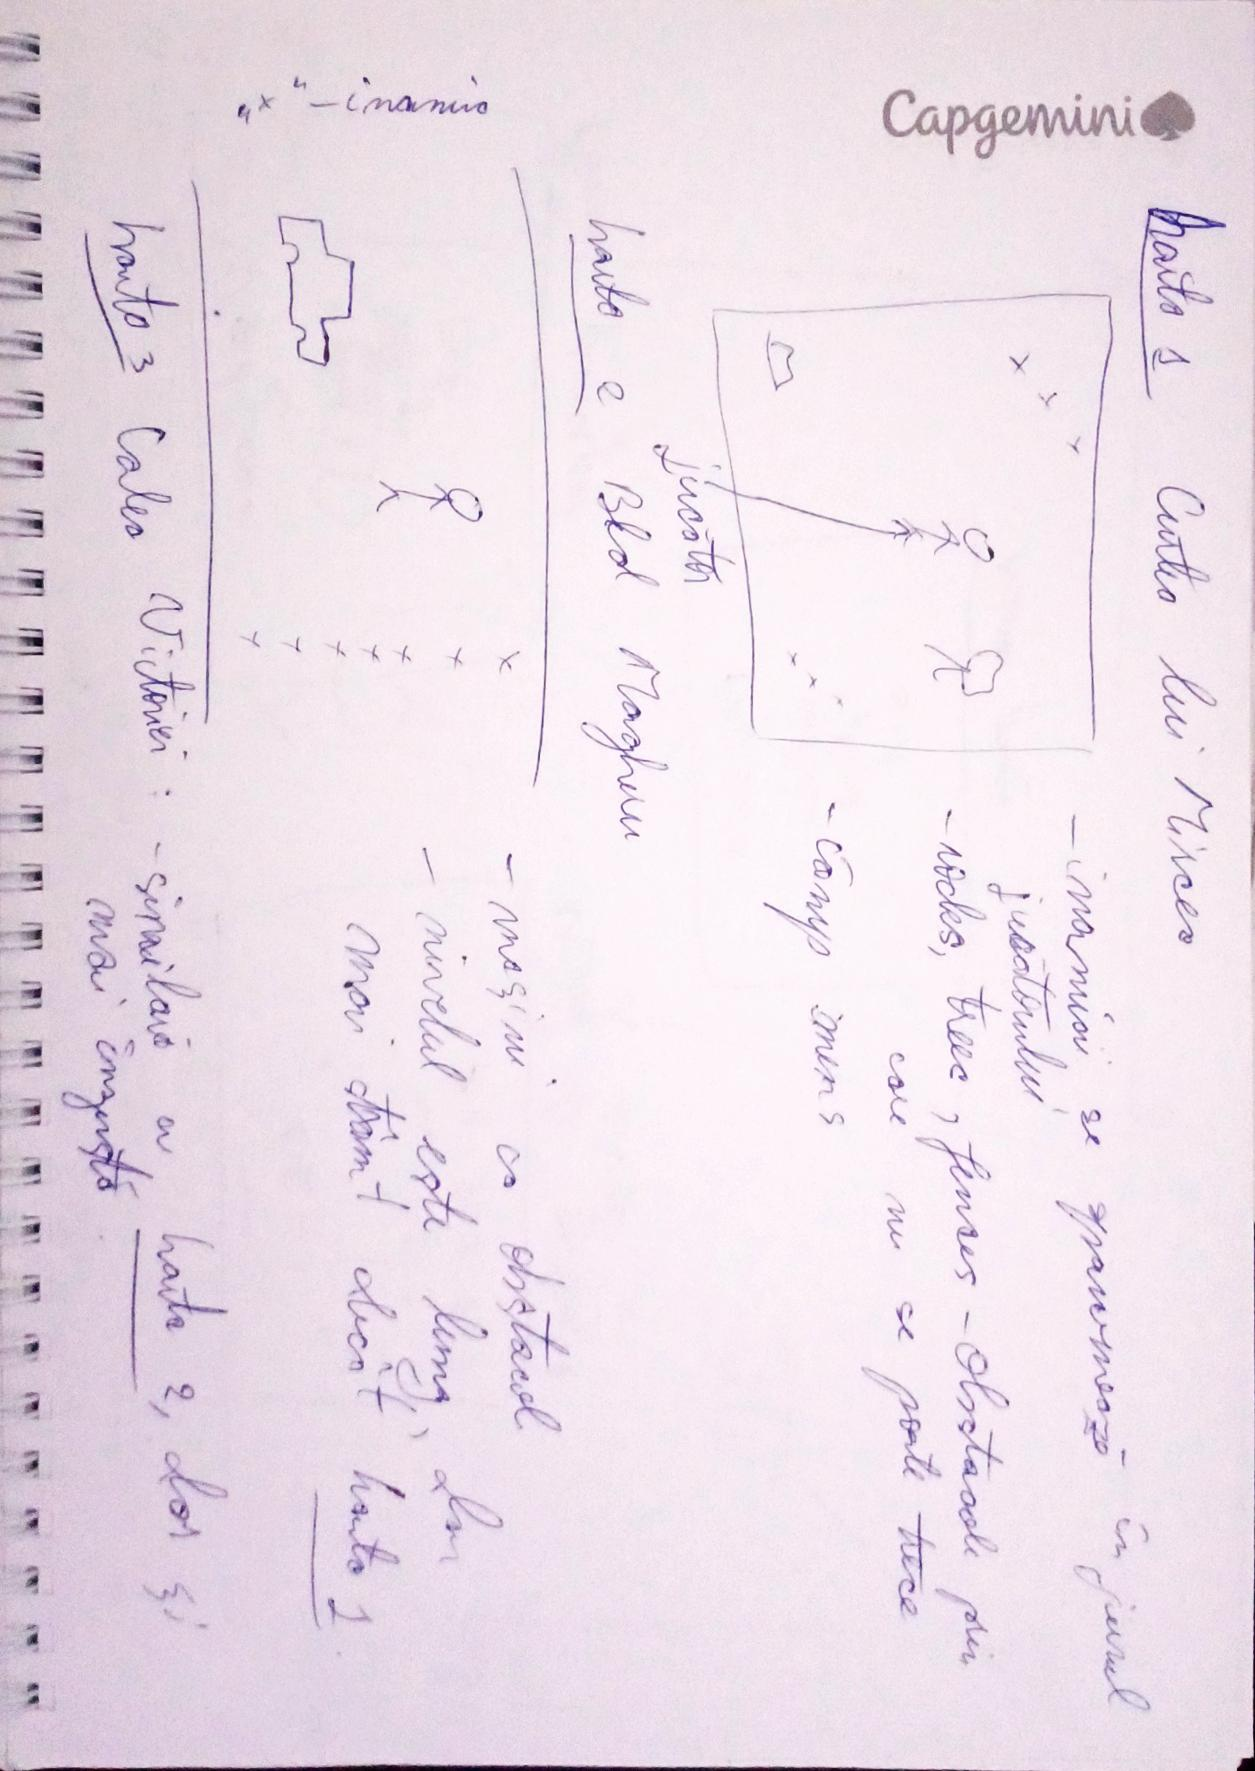
\includegraphics[width=0.55\textwidth, angle=90]{designing-levels}
        \centering
        \caption{Proiectarea nivelurilor}
    \end{figure}

    \emph{WizardGame 2} are următoarele niveluri:
    \begin{itemize}
        \item \emph{Curtea lui Mircea} --- un cămp larg, în care obstacolele sunt garduri,
        pietre și copaci, dar care în general oferă o libertate de mișcare crescută. Inamicii
        prezenți vor fi schelete, cranii zburătoare și zombie. Inamicii de tip boss vor fi
        \emph{Matei, the Profaned} și \emph{Adrian, the Crimson Undead}.
        \item \emph{Bulevardul Magheru} --- un nivel mai îngust, în care obstacolele vor fi
        mașini parcate. Inamicii prezenți vor fi schelete cu armură, zombie și fantome. Inamicii
        de tip boss vor fi \emph{Denis, the Cosmicbane} și \emph{Cezar, the Tătărașiborn Guardian}.
        \item \emph{Calea Victoriei} --- un nivel și mai îngust care va încapea în totalitate pe
        ecran în înălțime, dar nu în lățime. \emph{Cristian, the Necromancer of Neamț} va fi
        singurul inamic de tip boss, dar lupta cu el va fi în două etape.
    \end{itemize}

    În toate aceste nivele vor exista inamici de tip mini-boss care sunt versiuni mai mari și mai
    puternice a celor normali.

    Dificultatea va crește în fiecare nivel prin incluziunea inamicilor care apar după jumătatea
    timpului în nivelul anterior și prin creșterea puterii ataculurilor inamicilor.

    \section{Interfața grafică}

    \begin{figure}[H]
        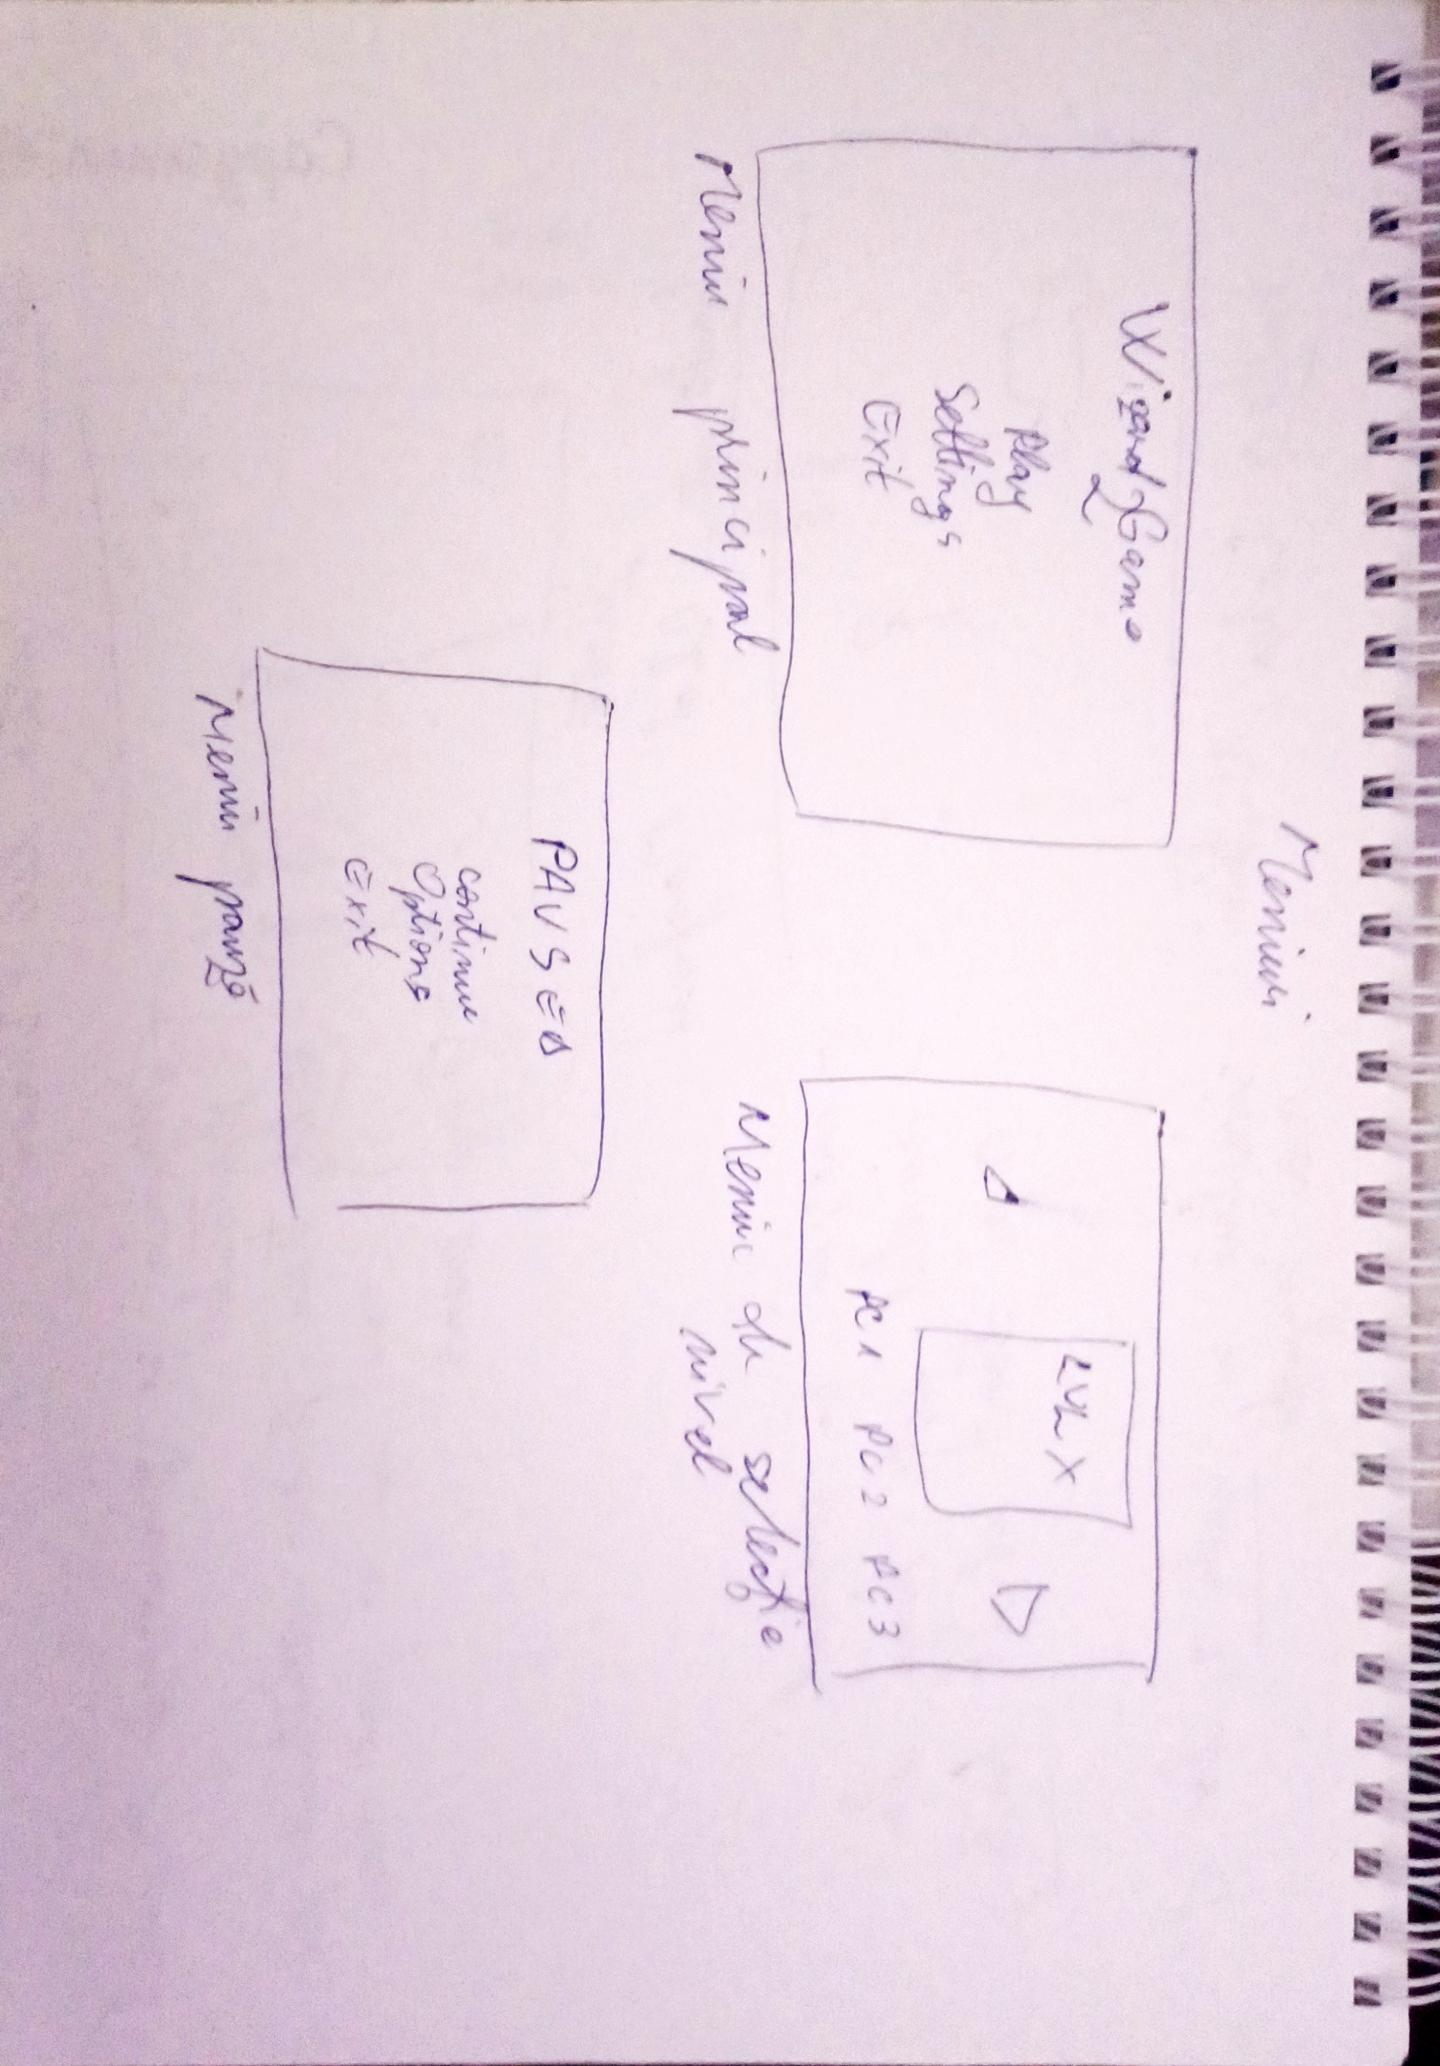
\includegraphics[width=0.45\textwidth, angle=90]{designing-menus}
        \centering
        \caption{Proiectarea meniurilor aplicației}
    \end{figure}

    Meniurile jocului sunt standard și proiectate pentru a fi intuitive pentru oricine a mai jucat
    jocuri. Interacțiunea cu elementele meniurilor se va realiza folosing cursorul mouse-ului, dar
    va fi permisă și folosirea tastelor, ca și în restul aplicațiilor grafice.

    \begin{figure}[H]
        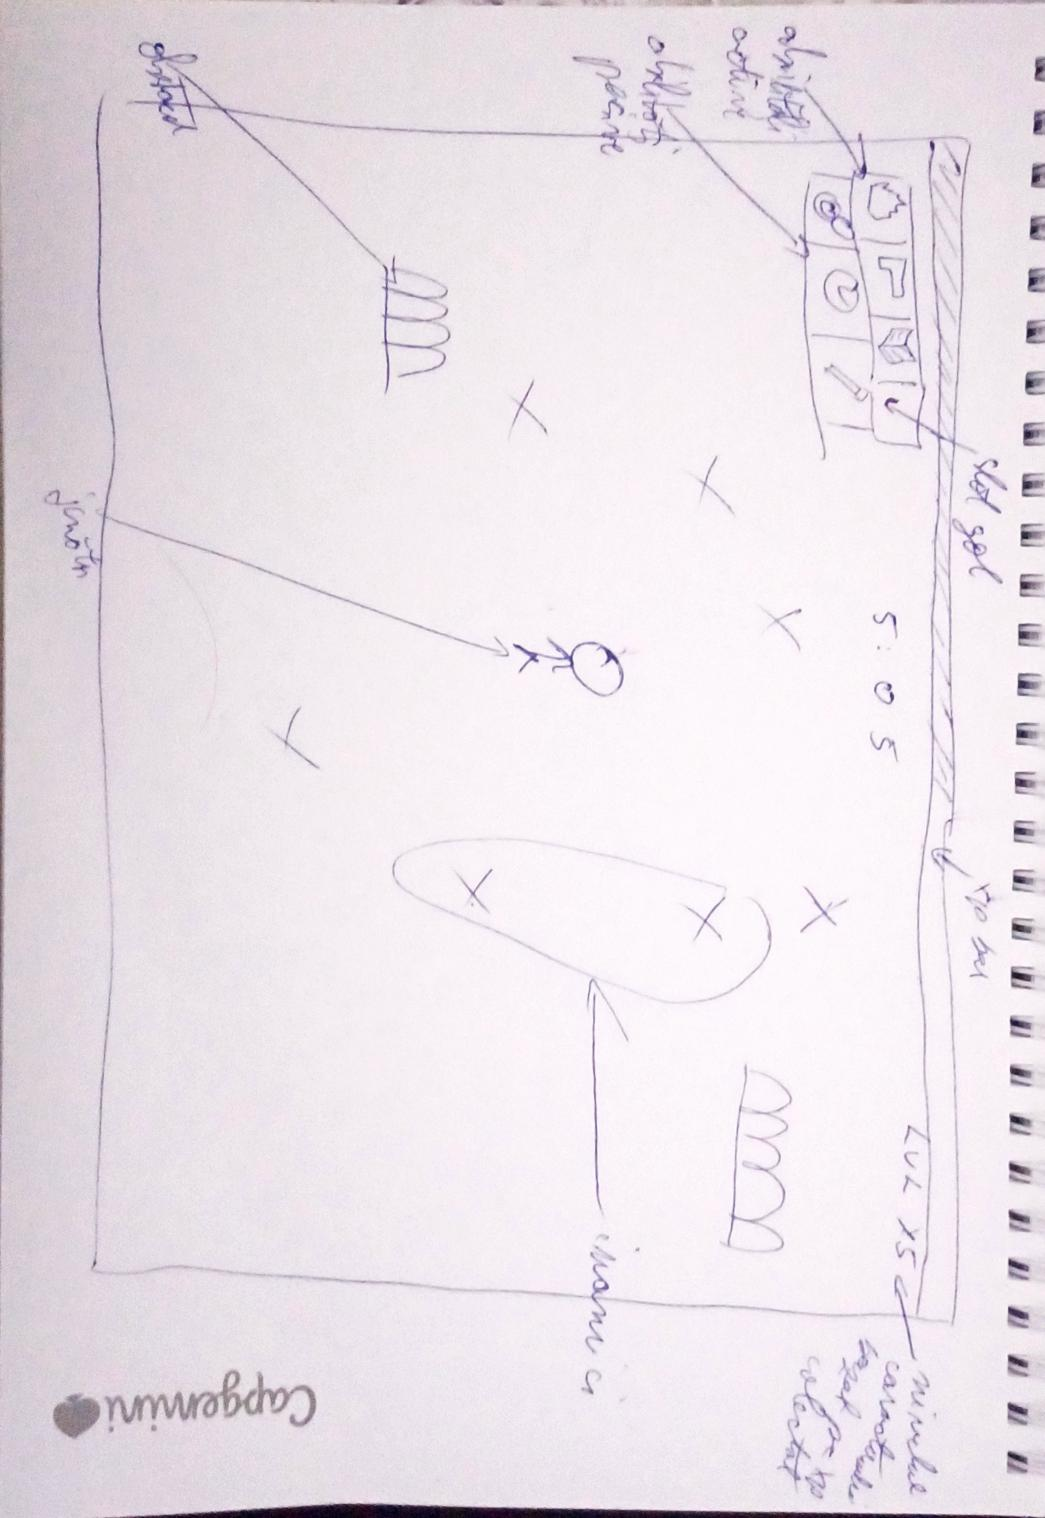
\includegraphics[width=0.45\textwidth, angle=90]{designing-level-ui}
        \centering
        \caption{Schița interfeței grafice într-un nivel}
    \end{figure}

    Interfața grafică dintr-un nivel a fost proiectată cu scopul de a nu distrage de
    la acțiunea principală, dar în același timp ea oferă informațiile esențiale de care are
    nevoie jucătorul.

    În general am urmat simplicitatea în proiectarea interfeței grafice, pentru a nu distrage
    jucătorul de la ce este important.

    \FloatBarrier
    \addcontentsline{toc}{section}{Anexa 1}
    \section*{Anexa 1}
    \label{sec:anexa1}
    Evenimentele \emph{WizardGame} se întâmplă cu 2 ani înainte de \emph{WizardGame 2}, în 1964,
    când \emph{Adrian, the Shaman of Neamț} anunță că va distruge Munții Carpați după ce tocmai
    a furat toate cărțile de vrăji ale vrăjitorilor români. Mircea, cunoscând vraja \emph{Fireball}
    în foarte multe detalii nu are nevoie de cărți magice pentru a folosi vraja, și decide să îl
    oprească pe Adrian, dar \emph{Matei}, senseiul său este doborât de mionionii lui Adrian.
    Jocul se termină prin moartea lui Adrian și salvarea Munților Carpați.

    \addcontentsline{toc}{section}{Bibliografie}
    \section*{Bibliografie}
    Jocul este inspirat conceptual și mecanic de jocurile \emph{Vampire Survivors}
    \href{https://store.steampowered.com/app/1794680/Vampire_Survivors/}{Steam} și
    \emph{Holocure} \href{https://kay-yu.itch.io/holocure}{itch.io}.

    Sprite-urile de pe pagina \pageref{sec:sprites} sunt realizate folosind tile-urile publicate
    pe următoare pagină web: \url{https://opengameart.org/content/dungeon-crawl-32x32-tiles}.


\end{document}
